%%%%%%%%%% PREAMBLE %%%%%%%%%%

%MNRAS style
\documentclass[fleqn,usenatbib]{mnras}
%default MNRAS packages
\usepackage{newtxtext,newtxmath}
\usepackage[T1]{fontenc}
\usepackage{ae,aecompl}
% user packages
\usepackage{graphicx}
\usepackage{amsmath}
\usepackage{amssymb}
\usepackage{dsfont}
%user commands
\newcommand{\acro}{TREVR}
\providecommand{\e}[1]{\ensuremath{\times10^{#1}}}

%%%%%%%%%%%%%%%%%%%%%%%%%%%%%%

%%%%%%%%%% TITLE PAGE %%%%%%%%%%

\title[]{\acro{}: Tree-based Reverse Ray Tracing 
in Gasoline}

\author[R. M. Woods et al.]{
R. M. Woods,
J. J. Grond, %\thanks{E-mail: grondjj@mcmaster.ca},
J. Wadsley %\thanks{E-mail:  wadsley@mcmaster.ca}
and H. M. P. Couchman
\\
Department of Physics and Astronomy, McMaster University, Hamilton, Ontario L8S
 4M1, Canada}

\date{Accepted XXX. Received YYY; in original form ZZZ}

\pubyear{2017}

\begin{document}
\label{firstpage}
\pagerange{\pageref{firstpage}--\pageref{lastpage}}
\maketitle

% Abstract of the paper
\begin{abstract}
%Temporarily commented out
%We present \acro{} (Fast Adaptive Hierarchical Radiative Transfer), a novel 
%algorithm for computing the radiation field in astrophysical simulations. 
%\acro{} prioritizes the ability to deal with a large number of sources and 
%computational speed over accuracy, while keeping equilibrium behaviour correct.
% The algorithm is based on a \emph{tree} data structure similar to many gravity
% solvers. This allows for computation of radiative transfer in 
%$\mathcal{O}(N_{\rm sink} \log N_{\rm source})$ time without absorption and 
%$\mathcal{O}(N_{\rm sink} \log N_{\rm source} \log{N})$ time with absorption. 
%Its tree based nature also allows it to scale well with number of processors 
%and be highly tunable in both speed and accuracy. A main feature of \acro{} is 
%the implementation of a refinement criteria based on the worst case optical 
%depth of a tree cell, allowing us to save cost whilst being confident in the 
%accuracy of our solution. The algorithm is also weakly dependent on the energy 
%band of radiation and the number of bands used, allowing for the radiation 
%fields of multiple bands to be computed on the fly with a negligible increase 
%in computational cost. We provide a suite of tests demonstrating the 
%algorithm's ability to accurately compute fluxes, ionization fronts and 
%shadows. We also analyze the algorithm's computational complexity, in how it 
%scales with the number of sources (star particles) and sinks (gas particles). 
%We also examine how the aforementioned refinement criterion's value affects 
%speed and accuracy. Finally, we will discuss strengths and shortcomings of this
% algorithm and how they constrain the niche of problems it can handle.
\end{abstract}

% Select between one and six entries from the list of approved keywords.
% Don't make up new ones.
\begin{keywords}
radiative transfer -- methods: numerical -- galaxies
\end{keywords}


%%%%%%%%%%%%%%%%%%%%%%%%%%%%%%

%%%%%%%%%% BODY OF PAPER %%%%%%%%%%

\section{INTRODUCTION}\label{sec:intro}

{\bf JW: This focusses a lot on observing but our primary interest is astrophysics.  Just adjust the balance to the paragraph more to physics.}
{\bf Does any other paper shorten Radiative Transfer to RT? To me it feels wrong to do that.}
Radiation is arguably the most important physical phenomenon in 
astrophysics. Almost all of the information we receive from space comes 
in the form of photons we detect on or around earth.  Understanding the process 
of radiative transfer (RT) is key in interpreting this information, as the 
photons are affected by the medium they travel through on the way to our 
telescopes and detectors. Interactions between photons and the medium along
 their paths do not only affect the photons themselves, but the matter as well.
 These interactions with baryons exchange energy and momentum, and also affect
 the excitation and ionization states of said baryons, thus determining the 
chemical and thermodynamic properties of the matter. This in turn makes 
radiation a driving factor in many of the physical processes we study.

Despite its importance, RT is treated rather poorly in many
 astrophysical simulations, usually as some imposed uniform background. This oversight 
is because RT is inherently a difficult problem. 
The full RT problem depends on 3 spatial dimensions, 2 
angular dimensions, frequency and time, and has a characteristic speed of $c$, 
the speed of light.  Gravity is also long range but RT is more complex because
 it depends on the intervening material.  A brute-force
numerical solution for RT would scale with the number resolution elements $N$ 
like $\mathcal{O}(N^{7/3})$.  Ideally, the scaling would be similar to current gravity and hydrodynamics
solvers ($\mathcal{O}(NlogN)$ or better).

We can separate numerical methods into two different
categories by looking at the classical RT equation 
\citep{mihalasMihalas84},

{\bf JW: I don't think we gain anything with all the arguments for every variable}
\begin{equation} \label{classicrt}
\left[ \frac{1}{c} \frac{\partial}{\partial t} + \mathbf{\hat{n} \cdot \nabla}
 \right] I\left(\mathbf{x}, \mathbf{\hat{n}}, t, \nu\right) = 
\epsilon\left(\mathbf{x}, \mathbf{\hat{n}}, t, \nu\right) - 
\alpha\left(\mathbf{x}, \mathbf{\hat{n}}, t, \nu\right) 
I\left(\mathbf{x}, \mathbf{\hat{n}}, t, \nu\right),
\end{equation}
where $I$, $\epsilon$ and $\alpha$ are the intensity, emissivity and extinction
 coefficient respectively which all depend on position $\mathbf{x}$, 
unit direction of light propagation $\mathbf{\hat{n}}$, time $t$ and frequency 
$\nu$. The difference comes from how different methods treat the speed of 
light $c$. For methods that use a finite $c$, which is often a 
reduced speed of light, the partial time derivative remains in equation 
\ref{classicrt} and the radiation field is advected or ``evolved''. Methods 
that solve the RT equation in this way, which we will call evolutionary 
methods, include moment methods like OTVET \citep{gnedinAbel01} and  RAMESE-RT 
\citep{rosdahlTeyssier15} as well as photon packet propagation methods like 
TRAPHIC \citep{pawlikSchaye08}, SPHRAY \citep{altayEt08} and SimpleX2 
\citep{paardekooperEt10}. On the other hand, in limit where $c$ is taken to be 
infinite, the partial time derivative in equation \ref{classicrt} goes to zero 
and the radiation field can be computed instantaneously. Methods that solve the
 RT equation in this way, which we will refer to as instantaneous methods, 
include forward ray tracers such as $\rm C^2Ray$ \citep{mellemaEt06a}, Moray 
\citep{wiseAbel11} and Fervent \citep{baczynskiEt15} as well as the limited reverse ray 
tracers such as TreeCol \citep{clarkEt12} and URCHIN \citep{altayTheuns13}.

All of these methods require simplifications to the full RT problem to make 
them feasible. These simplifications determine 
what types of problems they can solve. This 
makes comparing these methods on an equal footing somewhat confusing, as some 
authors state how their method scales with resolution elements in the context 
of the problem their RT method is meant to solve. For example, \cite{clarkEt12}
 state that their reverse ray tracer TreeCol scales with resolution elements 
like $\mathcal{O}(N\log{N})$. The specific problem they are trying to solve is 
the calculation of column densities via RT from background radiation, and thus
the number of sources of radiation they simulate is some small fixed number. 
They treat the number of sources as a constant factor in their scaling 
function, and so what is an $\mathcal{O}(N^2)$ method in the general case 
looks like a much more feasible method at first glance. For this reason we will
be very careful with scaling statements, using the number of radiation sources 
$N_{\rm source}$ and sinks $N_{\rm sink}$ where appropriate to make the 
limitations and possible uses of a given method clear.

Instantaneous methods come in the form of ray tracers. Ray tracers are the most
 simple, natural way to go about solving the RT problem. Forward ray tracers 
trace many rays outward from sources of radiation, similarly to the actual 
phenomena, in hope that they will intersect resolution elements for which the 
radiation field will be computed. Each source needs to compute a number of rays
 comparable to the number of resolution elements to ensure accuracy, 
meaning forward ray tracers scale with number of resolution elements like 
$\mathcal{O}(N_{\rm source} N_{\rm sink})$. This scaling limits forward ray 
tracers to problems with few sources to avoid $\mathcal{O}(N^2)$ like scaling. 
This also rules out the inclusion of scattering in the method as scatterings 
are treated as re-emission events and thus all sinks would have to be treated 
as sources as well. 

Recently there has been some focus on reverse ray tracing methods 
\citep{clarkEt12, altayTheuns13}. Reverse ray tracers trace rays from the sink 
particle directly to the sources. This way of tracing the rays has a couple of 
benefits over forward ray tracing. Firstly, tracing from the sinks guarantees 
the density distribution is well sampled as apposed to forward ray tracing 
where one would have to increase the number of rays per sink to guarantee 
accuracy. Put simply, radiation is computed exactly where it is needed. This 
is especially advantageous in smoothed particle hydrodynamics (SPH) 
simulations, as low density regions are represented by few SPH particles, and 
thus extra work is not done to resolve said regions. Another benefit is that 
sub time steps can be used. However, just performing a naive reverse ray trace 
does not negate $\mathcal{O}(N_{\rm source} N_{\rm sink})$ scaling with 
resolution elements, and so the inability to model many sources remains the 
most significant barrier current instantaneous methods face when trying to 
solve the general RT problem.

Evolutionary methods do not suffer from the linear dependence on number of 
sources. The main benefit of evolutionary methods is that they have no 
dependence on the number of sources, and just scale like $\mathcal{O}(N)$ with
the number of resolution elements, allowing them to handle large numbers of 
sources and scattering. Moment methods are limited to the optically thick 
diffusive limit. They also lack sharp directionality, resulting in poor shadows
behind optically thick objects. This also makes moment methods reliant on the 
partitioning of space into uniform grids. If implemented in a smooth particle 
hydrodynamics (SPH) like scheme, the lack of resolution elements in less dense 
regions would only exacerbate the directionality problem. 

Photon packet propagation methods, specifically TRAPHIC \citep{pawlikSchaye08},
 perform better in the optically thin regime. TRAPHIC introduces virtual 
particles (ViPs) to propagate their photon packets in less dense, optically 
thin regions lacking in SPH particles. They also preserve directionality quite 
well, however Monte Carlo aspects of how they propagate their photon packets 
introduce significant noise into their computed radiation field. Monte Carlo
 resampling is shown to reduce this noise but is quite expensive and 
deteriorates the initially sharp shadows. Both of these methods scale linearly 
with resolution elements as mentioned before, but are also forced to operate on
 every resolution element. In moment methods the radiation field for every 
grid cell needs to be computed, and in photon packet propagation methods the 
photon packets hop particle to particle. In the case of TRAPHIC, their $N$ is 
even greater than the number of SPH particles including the addition of ViPs. 
Regardless, TRAPHIC is arguably the best general RT method due to its ability 
to handle both the optically thick and thin regimes with feasible scaling.

We hope from this introduction to the state of the art in RT methods it is 
apparent that there is room for improvement. Although promising work has been 
done with reverse ray tracers like TreeCol, a general implementation of one has
 yet to be published. There is also the problem of scaling with sources in 
instantaneous methods. If this could be solved, instantaneous ray tracers could
 compete with the feasibility and improve upon the accuracy of evolutionary
 codes like TRAPHIC.

In this paper we introduce \acro{} (Tree-based Reverse Ray Tracing), a novel 
method that hopes to address all of the issues presented in the previous 
paragraph. \acro{} is a reverse ray tracer based on the \cite{barnesHut86} tree
 gravity solver. \acro{} is implemented in the SPH code Gasoline 
\citep{wadsleyEt03}, but we would like to note that the basic algorithm is not
 SPH or Gasoline specific, \acro{} only requires that the simulation volume be 
divided hierarchically in space. 

{\bf none of this below belong in an intro -- it is method }

A main feature of \acro{} is that sources can be merged via an opening  angle 
criteria similarly to the Barnes and Hut gravity method. This means that 
\acro{} scales with sources like $\mathcal{O}(\log N_{\rm source})$, 
alleviating the linear scaling with sources characteristic of other 
instantaneous RT methods. Being a reverse ray tracer enables us to easily merge
 sources, as sources interact with a single sink at a time. This is 
the first time source merging has been implemented in a reverse ray tracer, and
 thus \acro{} is the first general reverse ray tracer that can feasibly operate
 on all sources in a simulation and not just a small, fixed amount of 
background sources as in TreeCol and URCHIN.

\acro{} traces rays per each sink because it is a reverse ray tracer, this 
adds a linear dependence on the number of sinks. This coupled with source 
merging means \acro{} can solve the optically thin case 
$\mathcal{O}(N_{\rm sink} \log N_{\rm source})$ operations. The fact that
 \acro{} depends on a tree-data structure allows it to trace rays through an 
optically thick medium by traversing the sub-tree between the sink and source 
which is at most $\log N$ tree cells. This results in scaling with resolution
 elements in the optically thick case that goes like 
$\mathcal{O}(N_{\rm sink} \log N_{\rm source} \log N)$. This scaling in both 
the optically thin and thick case makes \acro{} a feasible method as it scales 
similarly to modern Gravity and Hydro solvers.

In the coming sections we will further explain the general method in section 
\ref{sec:method} and its implementation in section \ref{sec:implement}. Tests 
of scaling with resolution elements and the method's accuracy as a function of 
opening angle and refinement criteria will be presented in section 
\ref{sec:tests}. At the end of section \ref{sec:tests} we will do our best to 
compare \acro{} to other methods in common RT tests such as the Str\"{o}mgren
 sphere test and dense clump tests used in the \cite{ilievEt06} RT method 
comparison project. Finally, in section \ref{sec:dandc} we will discuss the 
method's merits and drawbacks to conclude where \acro{} fits in with other RT 
methods and what scientific problems it can solve.



\section{METHOD}\label{sec:method}
\section{Implementation}\label{sec:implement}
Temporarily commented out
%We now present the \acro{} algorithm. \acro{} prioritizes the ability to deal 
%with a large number of sources over high accuracy, though we still insist 
%equilibrium behaviour be correct. In order to accomplish this, we start by 
%making some simplifying assumptions to the radiative transfer equation
%\begin{equation}
%\label{eq:combtransfer}
%\frac{dI_\nu}{ds} = -\left(\alpha_\nu + \sigma_\nu)(I_\nu - S_\nu\right),
%\end{equation}
%where $\alpha_\nu$ and $\sigma_\nu$ are the specific absorption and scattering 
%coefficients respectively, $S_\nu$ is the combined source function for 
%absorption and scattering, and $I_\nu$ is the specific intensity.
%
%We can simplify \acro{} to only include absorption. This still allows us
%to treat scattering, as it can be expressed as an absorption followed by an 
%emission. For now though, we only account for absorption by treating star 
%particles as emitters and gas particles as absorbers. In the future one could 
%implement scattering by simply treating gas particles as emitters \textit{and}
%absorbers (more discussion on this in section \ref{sec:dandc}). This reduces 
%equation \ref{eq:combtransfer} to
%\begin{equation}
%\label{eq:absorbtransfer}
%\frac{dI_\nu}{d\tau_\nu} = -I_\nu + S_\nu,
%\end{equation}
%where $\tau_\nu$ is absorption-only optical depth and is defined as
%\begin{equation}
%\label{eq:tau}
%d\tau_\nu = \alpha_\nu ds = \rho \kappa_\nu ds,
%\end{equation}
%where $\rho$ is density and $\kappa_\nu$ is specific opacity due to absorption.
%
%It is useful to consider only absorption, as many astrophysical simulations 
%only model a single or few sources. This causes the emission coefficient to be 
%zero at most points. In our case we only consider star particles to be emitters,
% meaning we have a non emitting medium along a ray. This reduces equation 
%\ref{eq:absorbtransfer} by setting the source function to 0 and setting 
%$I_\nu$ to be the initial intensity from a single star particle $I_\nu(0)$ 
%\begin{equation}
%\label{eq:absorbsoln}
%I_\nu(\tau_\nu) = I_\nu(0)e^{-\tau_\nu}.
%\end{equation}
%This now allows us to turn the initial integral over all sources to a sum of
%diminished contributions from each star particle.
%
%We compute the radiation field as a flux magnitude, as this is the quantity most
% useful to applications of our algorithm. When expressed as a flux 
%\ref{eq:absorbsoln} becomes,
%\begin{equation}
%\label{eq:flux}
%F_\nu = \frac{L_\nu}{4\pi s^2} e^{-\tau_\nu},
%\end{equation}
%where $L_\nu$ is the specific luminosity of the star particle and $s$ is the 
%distance between the star particle and the absorbing gas particle. We can then 
%sum this equation over all contributing star particles to find the flux at 
%the gas particle in question. This summation is what \acro{} computes for all 
%gas-type SPH particles in a simulation, thus approximating the radiation field.
%
%Please note that \acro{} has been implemented in the Smoothed Particle 
%Hydrodynamics (SPH) code \textsc{Gasoline} \citep{wadsleyEt03}. However, 
%\acro{} is \emph{not} specific to \textsc{Gasoline} or SPH. We only require 
%that the simulation volume can be hierarchically partitioned in space.
%
%\subsection{The Optically Thin Regime}
%In the absence of absorbing material, the optical depth is zero and equation 
%\ref{eq:flux} becomes just $L/4\pi s^2$. This problem is almost identical to 
%gravity, and so we use the same tree-based technique as gravity to solve it. 
%The tree-based gravity solver of \citet{barnesHut86} has become commonplace in 
%astrophysical simulations 
%\citep{hubberEt11,wadsleyEt03,springelEt01,vineSigurdsson98,benz88}. Like the 
%Barnes \& Hut algorithm our optically thin method should scale with resolution
% elements like $\mathcal{O}(N\log{N})$. In our case the $N$ factor represents 
%the number of gas particles ($N_{\rm sink}$), and the $\log{N}$ factor 
%represents the number of emitting particles ($N_{\rm source}$). This means that
%for the optically thin case we should see scaling with number of sinks and 
%sources go as $\mathcal{O}(N_{\rm sink} \log{N_{\rm source}})$. 
%
%In our \textsc{Gasoline} implementation we use a binary tree. During the tree 
%build process we can compute useful average properties of tree cells such as 
%total luminosity, centre of luminosity, average density and average opacity 
%(the latter two are used in the optically thick regime). Computing the 
%radiation field is accomplished by traversing the tree structure. Receiving gas
% particles which live in the leaf nodes of the tree are looped over. An opening
% angle criterion, just as in gravity, is used to decide on how the gas 
%particles interact with the emitters.
%
%Note that we already have used early versions of this algorithm to
% investigate the effects of ionizing feedback on gas cooling in galaxies
%\citep{kannanEt14}.
%
%\subsection{The Optically Thick Regime}
%In the presence of absorbing material along the ray, we need to compute the 
%optical depth along said ray. To do this we traverse the tree from the 
%interacting nodes to their common parent node to build up the optical depth 
%along the ray. This is possible because the tree is partitioned in space, thus
%all intervening material should be contained in the sub-tree we traverse. Using
%the average properties computed in the tree build we can compute the optical 
%depth of a piece of the ray using the geometry of the cell and ray, and the 
%average density and opacity
%\begin{equation}
%\label{eq:taui}
%\tau_i = \bar{\rho_i} \bar{\kappa_i} s_i.
%\end{equation}
%The total optical depth is then summed up during the tree walk,
%\begin{equation}
%\label{eq:tausum}
%\tau = \sum_i \tau_i,
%\end{equation}
%giving us everything needed to evaluate equation \ref{eq:flux}. Because of this
% extra tree walk another $\log N$ factor can be added to the scaling equation 
%and so we would expect the scaling with resolution elements to now look like
%$\mathcal{O} (N_{\rm sink} \log N_{\rm source} \log N)$. This algorithm is 
%depicted in the left half of figure \ref{fig:tree}
%
%Since we are calculating the radiation field at the receiving cell we are doing
% a process similar to a reverse ray trace, like URCHIN \citep{altayTheuns13}. 
%One advantage of reverse ray tracing is that rays are associated with with 
%sinks rather than the source. Dense regions near the sink and source are 
%therefore automatically well sampled and radiative transfer is computed 
%exactly where it needs to be. Another benefit is that the simulation can make 
%use of sub time steps. The problem with this simple method is that as the 
%tree is traversed upwards the volume elements become larger and accuracy can be
% lost. That makes this algorithm very efficient at computing the radiation 
%field for uniform density and opacity distributions, but highly inaccurate when
% dealing with sharp density and opacity gradients along the ray. To handle 
%these situations a method of refinement is needed.
%
%\subsection{Refinement}
%Refinement is a straightforward addition to the algorithm. At a point in the 
%tree walk where the average properties of the cell would be considered, we 
%check to see if the current cell passes some refinement criteria. If the cell 
%passes the criteria to refine, rather than using the average properties we 
%recursively check the cell's children until the criteria fails building a 
%better resolved  section of the ray. This addition to the algorithm is depicted
% in the right half of figure \ref{fig:tree}
%\begin{figure*}
%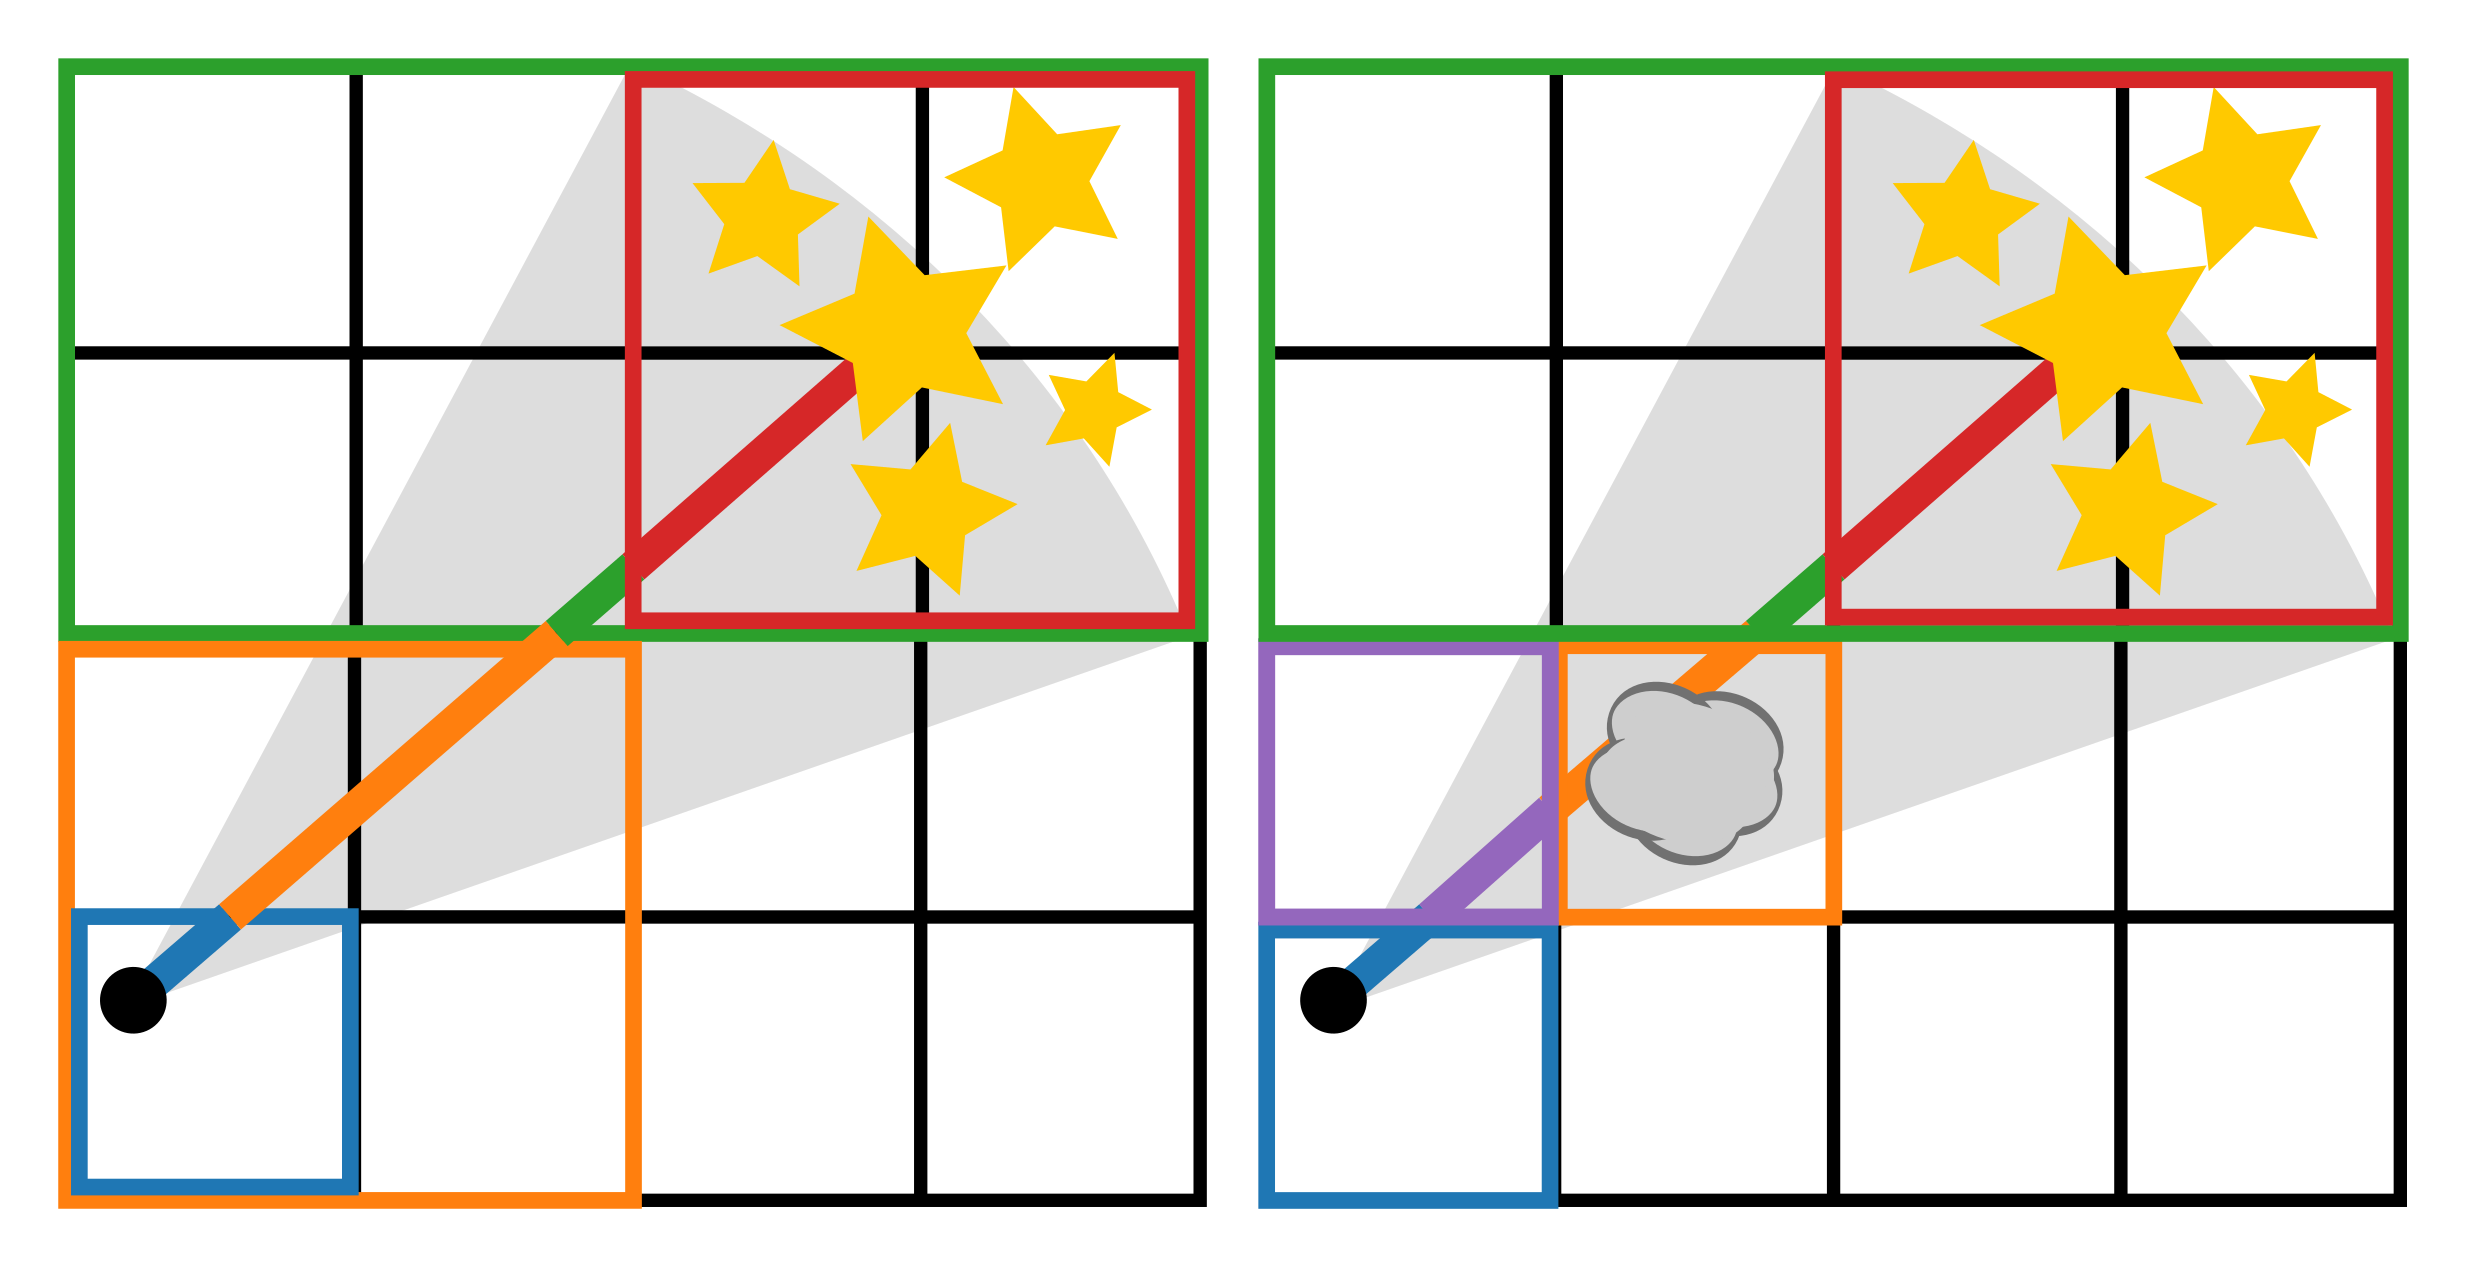
\includegraphics[width=1\linewidth]{Figures/algorithm.png}
%\caption{Depiction of the \acro{} algorithm with and without the need for 
%refinement (left and right respectively.)}
%\label{fig:tree}
%\end{figure*}
%
%Difficulty comes in choosing a refinement criteria that is both accurate and 
%efficient. Ideally, the criteria should be true when an average optical depth 
%in a region may not be accurate to the true distribution, such as a clumpy 
%medium where the average opacity is much higher than the ``effective'' opacity
% \citep{hegmanKegel03,varosiDwek99}.
%
%Our choice of refinement criteria is based on optical depth, and is unique to 
%the \acro{} algorithm. Consider two rays through a large cell (see figure 
%\ref{fig:refine}, note that this description is simplified to 2D).
%\begin{figure}
%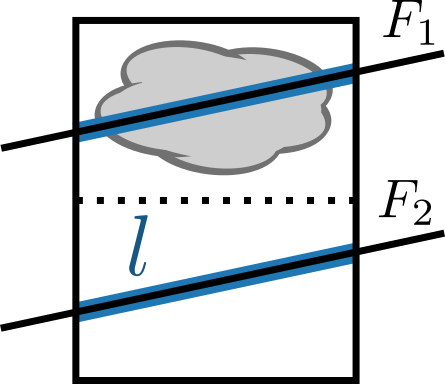
\includegraphics[width=0.45\textwidth]{Figures/refine.png}
%\caption{refine.pdf}
%\label{fig:refine}
%\end{figure}
%These rays represent what the case would be if the properties of the children 
%were used instead of the parent cell. We can calculate the minimum and maximum 
%absorption coefficients $\alpha_{\rm min}$ and $\alpha_{\rm max}$, via their 
%average density and opacity values computed during the tree build. This 
%multiplied by the intersection $l$, gives us the minimum and maximum optical 
%depths, $\tau_{\rm min}$ and $\tau_{\rm max}$. We can then test the following 
%refinement criteria
%\begin{equation}
%\tau_{\rm refine} < \tau_{\rm max} - \tau_{\rm min},
%\end{equation}
%and refine if it is true. The fractional error in flux for a chosen value of 
%$\tau_{\rm refine}$ is 
%\begin{equation}
%{\rm Fractional Error} = \frac{F_1-F_2}{F_1} \leq 1 - e^{(-\tau_{\rm max} - 
%\tau_{\rm min})} < \tau_{\rm refine},
%\end{equation}
%for small $\tau$, making the refinement criteria a convenient choice of 
%parameter for guaranteeing accuracy.  This criteria is conservative, as it 
%assumes the worst case difference in optical depth. We suspect there is room 
%for improvement in terms of efficiency.
%
%If very high accuracy is required, sub-leaf node refinement is possible. If a 
%leaf was reached during refinement and still passes the refinement criteria, 
%the individual particles in the leaf can be considered. A ray tracing scheme 
%through the cell similar to SPHRay \citep{altayEt08} can be performed. 
%The machinery to do this is implemented in \acro{}.
%
%\subsection{Cosmological Background Radiation}
%In order to treat cosmological simulations properly we must account for the 
%radiation coming from the rest of the universe outside of the simulation 
%volume. Most current codes apply a constant UV field to the entire box, 
%essentially the lowest order approximation possible. Some specialized codes 
%like URCHIN \citep{altayTheuns13} do a reverse ray trace to the edge of the 
%box, where the background flux is assumed to be coming from. Others, such as 
%TRAPHIC \citep{pawlikSchaye08} allow their ray trace to be periodic. We believe
% that this periodic treatment is problematic for reasons we will explain at the
% end of this subsection. 
%
%Instead, we have implemented a method involving ``background sources''. 
%``Background'' particles are distributed in a spiral pattern on the surface of 
%a sphere at the very edge of the simulation volume (or at a large distance if 
%required) and the number of sources can be varied to match the required angular
% resolution  of the background. Finding the flux at the centre of a sphere of 
%sources is a problem akin to Newton's Shell Theorem. However, because the 
%intensity does not cancel like force, the solution differs and is as follows:
%\begin{equation}\label{eq:cosmofield}
%F(r) = \frac{L}{8\pi R} \ln \left(\frac{R+r}{R-r}\right),
%\end{equation}
%where $L$ is the total luminosity of the emitting shell, $R$ is the radius of 
%the sphere and $r$ is the radius the flux is being computed at. The shape of 
%the function can be seen if Figure \ref{fig:cosmofield}
%\begin{figure}
%\label{fig:cosmofield}
%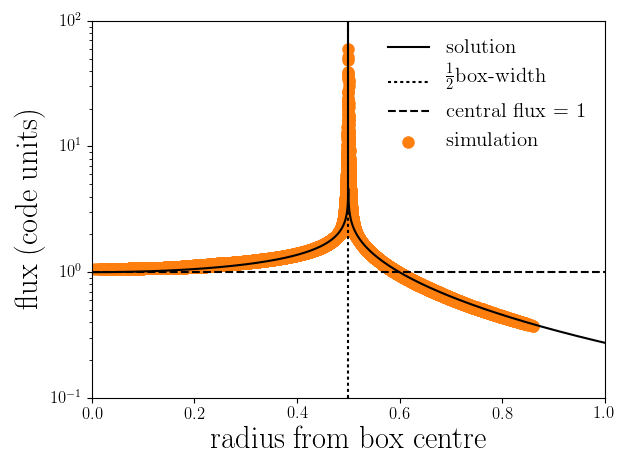
\includegraphics[width=0.5\textwidth]{Figures/cosmofield.png}
%\caption{The distribution of flux that particles receive due to the 
%cosmological background sources when distributed in a spherical shell on at the
% edge of the simulation box. Note that the value of the flux at the centre can
% be easily scaled by simply scaling $L$, the luminosity of all sources on the 
%sphere. The important property is the near constant flux at small radii. In
% this example, we have used 1024 background sources. The number of sources 
%determines the width of the peak.}
%\end{figure}
%where we have plotted the flux as a function of radius for a homogeneous,
%optically thin test volume.
%
%We note that due to the logarithm in equation \ref{eq:cosmofield}, the flux is
% nearly constant at small radii. Since most cosmological zoom in simulations 
%only consider gas at a fairly small radius, this setup of background sources is
% an acceptable method to provide a cosmological background flux. A benefit of
% this method is that we can use all of the existing machinery described in the 
%methods section, and only have to add temporary background star particles as 
%the source of the background radiation. This way, there is no need to create 
%periodic copies of the simulation volume. **explain <-this here**
%
\section{CODE TESTS}\label{sec:tests}

\section{DISCUSSION AND CONCLUSION}\label{sec:dandc}

\section*{Acknowledgements}

%%%%%%%%%%%%%%%%%%%%%%%%%%%%%%

%%%%%%%%%% REFERENCES %%%%%%%%%%

\bibliographystyle{mnras}
\bibliography{references}

%%%%%%%%%%%%%%%%%%%%%%%%%%%%%%

%%%%%%%%%% APPENDICES %%%%%%%%%%

\appendix

%%%%%%%%%%%%%%%%%%%%%%%%%%%%%%

\bsp
\label{lastpage}
\end{document}

%%%%%%%%%% FIN %%%%%%%%%%
